\documentclass[border=5pt]{standalone}
\usepackage{tikz}
\usepackage{pgfplots}
\pgfplotsset{compat=1.18}
\usepackage{amsmath,amssymb,amsfonts,bm}
\usepackage{xcolor}

% BRAND colors
\definecolor{tiger}{HTML}{FF5A00}
\definecolor{fire}{HTML}{FF4D00}
\definecolor{flicker}{HTML}{DC4B07}
\definecolor{steel}{HTML}{878F92}
\definecolor{gunmetal}{HTML}{122128}
\definecolor{panel}{HTML}{202E35}

% FIGURE colors
\definecolor{dark_navy}{HTML}{122128}
\definecolor{forgis_orange}{HTML}{FF5A00}
\definecolor{forgis_fire}{HTML}{FF4D00}
\definecolor{forgis_flicker}{HTML}{DC4B07}
\definecolor{blue}{HTML}{3A7BD5}
\definecolor{green}{HTML}{2ECC71}
\definecolor{panelbg}{HTML}{F0F4F8}
\definecolor{warm_amber}{HTML}{FFF3CD}

% LEVEL colors
\definecolor{L1bg}{HTML}{FCF0E0}
\definecolor{L1border}{HTML}{FB9E6C}
\definecolor{L2bg}{HTML}{FCF0E0}
\definecolor{L2border}{HTML}{FF7F3A}
\definecolor{L3bg}{HTML}{FCF0E0}
\definecolor{L3border}{HTML}{FF5A00}
\definecolor{L4bg}{HTML}{FCF0E0}
\definecolor{L4border}{HTML}{81360F}

\usetikzlibrary{arrows.meta, positioning, calc, fit, shapes.geometric, 
  decorations.pathreplacing, backgrounds, patterns, shadows}

\begin{document}
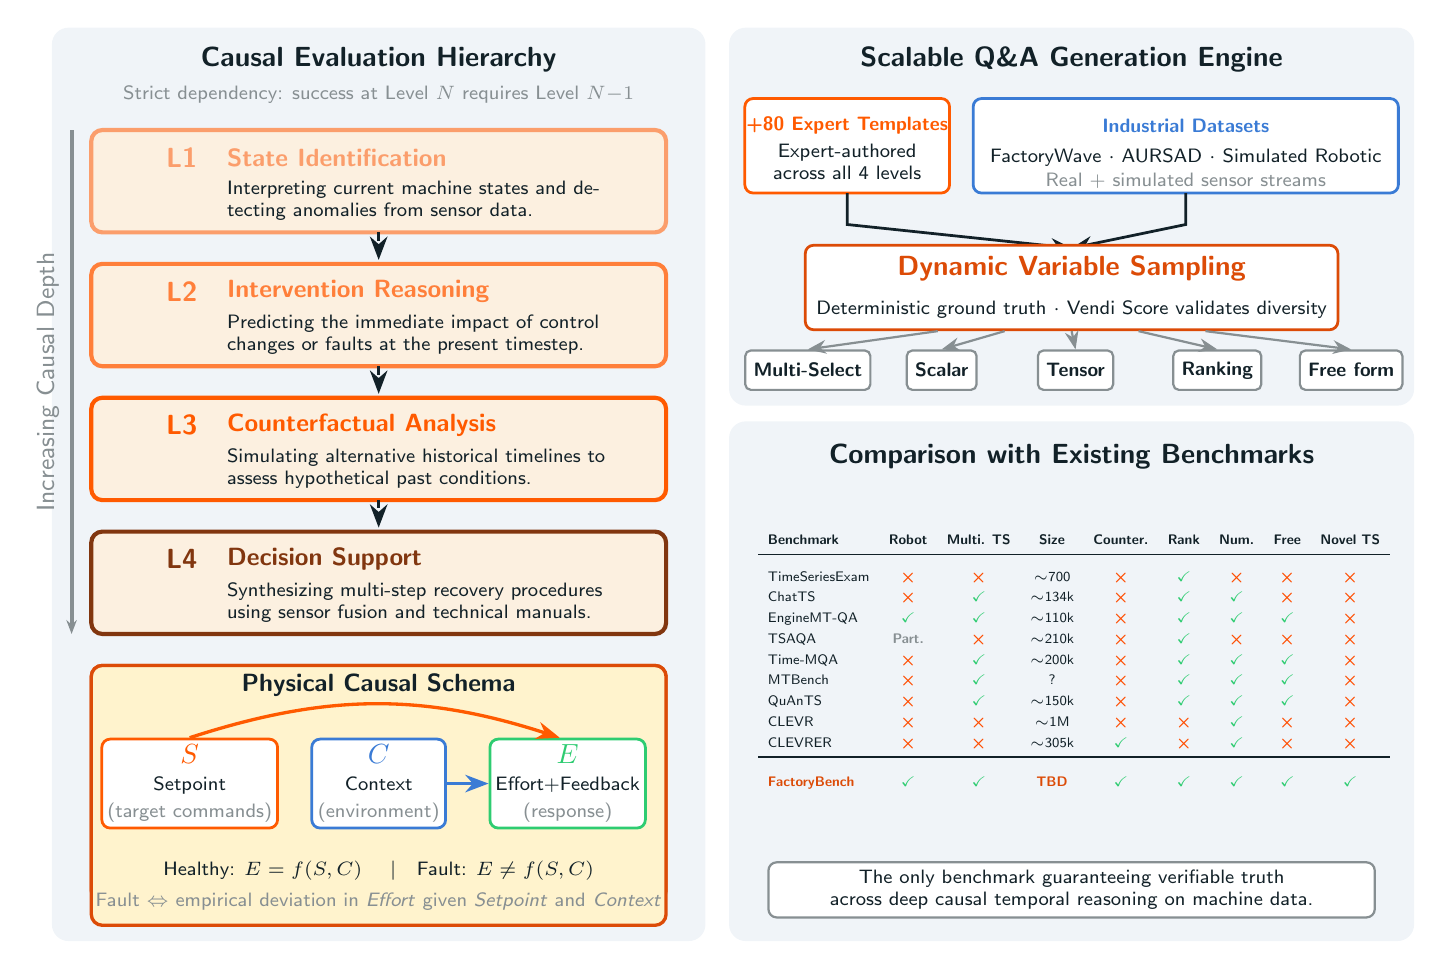
\begin{tikzpicture}[
  every node/.style={font=\sffamily},
  >=Stealth
]

% ====== TITLE ======
% \node[font=\sffamily\bfseries\Large, text=gunmetal] at (8.5, 16.8) 
%   {\textcolor{forgis_orange}{FactoryBench}: Four-Level Causal Evaluation Hierarchy};
% \node[font=\sffamily\small, text=steel] at (8.5, 16.2) 
%   {Rigorous QA benchmark for LLM agents on causal machine understanding with industrial time-series data};

% ====== LEFT COLUMN: HIERARCHY ======
% Background panel
\begin{scope}
\fill[panelbg, rounded corners=6pt] (-0.5, 4.0) rectangle (7.8, 15.6);
\node[font=\sffamily\bfseries\normalsize, text=gunmetal] at (3.65, 15.2) 
  {Causal Evaluation Hierarchy};
\node[font=\sffamily\scriptsize, text=steel] at (3.65, 14.75) 
  {Strict dependency: success at Level $N$ requires Level $N{-}1$};

% --- L1 ---
\fill[L1bg, rounded corners=4pt] (0.0, 13.0) rectangle (7.3, 14.3);
\draw[L1border, line width=1.5pt, rounded corners=4pt] (0.0, 13.0) rectangle (7.3, 14.3);
\node[font=\sffamily\bfseries, text=L1border] at (1.15, 13.95) {L1};
\node[font=\sffamily\bfseries\small, text=L1border, anchor=west] at (1.6, 13.95) {State Identification};
\node[font=\sffamily\scriptsize, text=gunmetal, text width=5.0cm, anchor=west] at (1.6, 13.4) 
  {Interpreting current machine states and detecting anomalies from sensor data.};

% --- L2 ---
\fill[L2bg, rounded corners=4pt] (0.0, 11.3) rectangle (7.3, 12.6);
\draw[L2border, line width=1.5pt, rounded corners=4pt] (0.0, 11.3) rectangle (7.3, 12.6);
\node[font=\sffamily\bfseries, text=L2border] at (1.15, 12.25) {L2};
\node[font=\sffamily\bfseries\small, text=L2border, anchor=west] at (1.6, 12.25) {Intervention Reasoning};
\node[font=\sffamily\scriptsize, text=gunmetal, text width=5.0cm, anchor=west] at (1.6, 11.7) 
  {Predicting the immediate impact of control changes or faults at the present timestep.};

% --- L3 ---
\fill[L3bg, rounded corners=4pt] (0.0, 9.6) rectangle (7.3, 10.9);
\draw[L3border, line width=1.5pt, rounded corners=4pt] (0.0, 9.6) rectangle (7.3, 10.9);
\node[font=\sffamily\bfseries, text=L3border] at (1.15, 10.55) {L3};
\node[font=\sffamily\bfseries\small, text=L3border, anchor=west] at (1.6, 10.55) {Counterfactual Analysis};
\node[font=\sffamily\scriptsize, text=gunmetal, text width=5.0cm, anchor=west] at (1.6, 10.0) 
  {Simulating alternative historical timelines to assess hypothetical past conditions.};

% --- L4 ---
\fill[L4bg, rounded corners=4pt] (0.0, 7.9) rectangle (7.3, 9.2);
\draw[L4border, line width=1.5pt, rounded corners=4pt] (0.0, 7.9) rectangle (7.3, 9.2);
\node[font=\sffamily\bfseries, text=L4border] at (1.15, 8.85) {L4};
\node[font=\sffamily\bfseries\small, text=L4border, anchor=west] at (1.6, 8.85) {Decision Support};
\node[font=\sffamily\scriptsize, text=gunmetal, text width=5.0cm, anchor=west] at (1.6, 8.3) 
  {Synthesizing multi-step recovery procedures using sensor fusion and technical manuals.};

% --- Dependency arrows ---
\draw[gunmetal, line width=1.2pt, ->, dashed] (3.65, 13.0) -- (3.65, 12.65);
\draw[gunmetal, line width=1.2pt, ->, dashed] (3.65, 11.3) -- (3.65, 10.95);
\draw[gunmetal, line width=1.2pt, ->, dashed] (3.65, 9.6) -- (3.65, 9.25);

% --- Difficulty arrow on the side ---
\draw[steel, line width=1.5pt, -{Stealth[length=5pt]}] (-0.25, 14.3) -- (-0.25, 7.9);
\node[font=\sffamily\small, text=steel, rotate=90] at (-0.55, 11.1) {Increasing Causal Depth};

\fill[warm_amber, rounded corners=4pt] (0.0, 4.5) rectangle (7.3, 7.5);
\draw[flicker, line width=1.2pt, rounded corners=4pt] (0.0, 4.5) rectangle (7.3, 7.5);

% ====== Physical Causal Schema ======
\fill[warm_amber, rounded corners=4pt] (0.0, 4.2) rectangle (7.3, 7.5);
\draw[flicker, line width=1.2pt, rounded corners=4pt] (0.0, 4.2) rectangle (7.3, 7.5);

\node[font=\sffamily\bfseries\small, text=gunmetal] at (3.65, 7.25) {Physical Causal Schema};

\tikzset{
  causalNode/.style={
    fill=white, rounded corners=3pt, align=center,
    minimum width=1.7cm, minimum height=1.0cm, inner sep=2pt
  }
}

\node[causalNode, draw=forgis_orange, line width=1pt] (nodeS) at (1.25, 6.0) {
  \textbf{\textcolor{forgis_orange}{$S$}}\\[-0.5ex]
  \scriptsize\textcolor{gunmetal}{Setpoint}\\[-0.5ex]
  \scriptsize\textcolor{steel}{(target commands)}
};

\node[causalNode, draw=blue, line width=1pt] (nodeC) at (3.65, 6.0) {
  \textbf{\textcolor{blue}{$C$}}\\[-0.5ex]
  \scriptsize\textcolor{gunmetal}{Context}\\[-0.5ex]
  \scriptsize\textcolor{steel}{(environment)}
};

\node[causalNode, draw=green, line width=1pt] (nodeE) at (6.05, 6.0) {
  \textbf{\textcolor{green}{$E$}}\\[-0.5ex]
  \scriptsize\textcolor{gunmetal}{Effort+Feedback}\\[-0.5ex]
  \scriptsize\textcolor{steel}{(response)}
};

\draw[forgis_orange, line width=1.2pt, ->] 
  (nodeS.north) to[bend left=18] ([xshift=-0.1cm]nodeE.north);

\draw[blue, line width=1.2pt, ->] (nodeC.east) -- (nodeE.west);

\node[font=\sffamily\scriptsize, text=gunmetal] at (3.65, 4.9) 
  {Healthy: $E = f(S, C)$ \quad \textbar \quad Fault: $E \neq f(S, C)$};

\node[font=\sffamily\scriptsize, text=steel] at (3.65, 4.5)
  {Fault $\Leftrightarrow$ empirical deviation in \textit{Effort} given \textit{Setpoint} and \textit{Context}};
\end{scope}

% ====== RIGHT COLUMN: GENERATION + RESULTS ======
% --- Q&A Generation Engine ---
\begin{scope}[xshift=-0.4cm]
\fill[panelbg, rounded corners=6pt] (8.5, 10.8) rectangle (17.2, 15.6);
\node[font=\sffamily\bfseries\normalsize, text=gunmetal] at (12.85, 15.2) 
  {Scalable Q\&A Generation Engine};

% Template box
\fill[white, rounded corners=3pt] (8.7, 13.5) rectangle (11.3, 14.7);
\draw[forgis_orange, line width=1pt, rounded corners=3pt] (8.7, 13.5) rectangle (11.3, 14.7);
\node[font=\sffamily\bfseries\scriptsize, text=forgis_orange] at (10.0, 14.35) {+80 Expert Templates};
\node[font=\sffamily\scriptsize, text=gunmetal, text width=2.4cm, align=center] at (10.0, 13.9) 
  {Expert-authored across all 4 levels};

% Datasets box
\fill[white, rounded corners=3pt] (11.6, 13.5) rectangle (17.0, 14.7);
\draw[blue, line width=1pt, rounded corners=3pt] (11.6, 13.5) rectangle (17.0, 14.7);
\node[font=\sffamily\bfseries\scriptsize, text=blue] at (14.3, 14.35) {Industrial Datasets};
\node[font=\sffamily\scriptsize, text=gunmetal] at (14.3, 13.95) {FactoryWave $\cdot$ AURSAD $\cdot$ Simulated Robotic};
\node[font=\sffamily\scriptsize, text=steel] at (14.3, 13.65) {Real + simulated sensor streams};

% Arrow down
\draw[gunmetal, line width=1pt, ->] (10.0, 13.5) -- (10.0, 13.1) -- (12.85, 12.8);
\draw[gunmetal, line width=1pt, ->] (14.3, 13.5) -- (14.3, 13.1) -- (12.85, 12.8);

% Dynamic sampling box
\node[
  draw=flicker, fill=white, line width=1pt, rounded corners=3pt, 
  align=center, inner sep=4pt, minimum width=4.7cm
] (sampling) at (12.85, 12.3) {
  \textbf{\textcolor{flicker}{Dynamic Variable Sampling}}\\[0.5ex]
  \scriptsize\textcolor{gunmetal}{Deterministic ground truth $\cdot$ Vendi Score validates diversity}
};

% Output formats
\tikzset{
  outbox/.style={
    draw=steel, line width=0.8pt, fill=white, rounded corners=2pt,
    font=\sffamily\scriptsize\bfseries, text=gunmetal, 
    minimum height=0.5cm, inner sep=3pt, align=center
  }
}

\node[outbox] (ms)      at (9.5,   11.25) {Multi-Select};
\node[outbox] (escalar) at (11.2, 11.25) {Scalar};
\node[outbox] (tensor)  at (12.9, 11.25) {Tensor};
\node[outbox] (rank)    at (14.7, 11.25) {Ranking};
\node[outbox] (open)    at (16.4,  11.25) {Free form};

\draw[steel, line width=0.8pt, ->] ([xshift=-1.7cm]sampling.south)  -- (ms.north);
\draw[steel, line width=0.8pt, ->] ([xshift=-0.85cm]sampling.south) -- (escalar.north);
\draw[steel, line width=0.8pt, ->] (sampling.south)                 -- (tensor.north); 
\draw[steel, line width=0.8pt, ->] ([xshift=0.85cm]sampling.south)  -- (rank.north);
\draw[steel, line width=0.8pt, ->] ([xshift=1.7cm]sampling.south)   -- (open.north);

\end{scope}

% ====== WHY FACTORYBENCH (COMPARISON MATRIX) ======
\begin{scope}[xshift=-0.4cm]
\fill[panelbg, rounded corners=6pt] (8.5, 4.0) rectangle (17.2, 10.6);
\node[font=\sffamily\bfseries\normalsize, text=gunmetal] at (12.85, 10.15) 
  {Comparison with Existing Benchmarks};

\def\cmark{\textcolor{green}{$\bm{\checkmark}$}}
\def\xmark{\textcolor{forgis_fire}{$\bm{\times}$}}
\def\pmark{\textcolor{steel}{\textbf{Part.}}}

\node[font=\sffamily\tiny, text=gunmetal, inner sep=0pt, align=center] at (12.85, 7.55) {
  \renewcommand{\arraystretch}{1.25}
  \setlength{\tabcolsep}{3.5pt}
  \begin{tabular}{l c c c c c c c c}
    \textbf{Benchmark} & \textbf{Robot} & \textbf{Multi. TS} & \textbf{Size} & \textbf{Counter.} & \textbf{Rank} & \textbf{Num.} & \textbf{Free} & \textbf{Novel TS} \\[0.5ex]
    \hline\\[-1.5ex]
    TimeSeriesExam & \xmark & \xmark & $\sim$700 & \xmark & \cmark & \xmark & \xmark & \xmark \\
    ChatTS & \xmark & \cmark & $\sim$134k & \xmark & \cmark & \cmark & \xmark & \xmark \\
    EngineMT-QA & \cmark & \cmark & $\sim$110k & \xmark & \cmark & \cmark & \cmark & \xmark \\
    TSAQA & \pmark & \xmark & $\sim$210k & \xmark & \cmark & \xmark & \xmark & \xmark \\
    Time-MQA & \xmark & \cmark & $\sim$200k & \xmark & \cmark & \cmark & \cmark & \xmark \\
    MTBench & \xmark & \cmark & ? & \xmark & \cmark & \cmark & \cmark & \xmark \\
    QuAnTS & \xmark & \cmark & $\sim$150k & \xmark & \cmark & \cmark & \cmark & \xmark \\
    CLEVR & \xmark & \xmark & $\sim$1M & \xmark & \xmark & \cmark & \xmark & \xmark \\
    CLEVRER & \xmark & \xmark & $\sim$305k & \cmark & \xmark & \cmark & \xmark & \xmark \\[0.5ex]
    \hline\\[-1ex]
    \textbf{\textcolor{forgis_flicker}{FactoryBench}} & 
    \cmark & \cmark & \textbf{\textcolor{forgis_flicker}{TBD}} & 
    \cmark & \cmark & \cmark & 
    \cmark & \cmark \\
  \end{tabular}
};

\fill[white, rounded corners=3pt] (9.0, 4.3) rectangle (16.7, 5.0);
\draw[steel, line width=0.8pt, rounded corners=3pt] (9.0, 4.3) rectangle (16.7, 5.0);
\node[font=\sffamily\scriptsize, text=gunmetal, align=center] at (12.85, 4.65) 
  {The only benchmark guaranteeing verifiable truth \\ across deep causal temporal reasoning on machine data.};

\end{scope}

\end{tikzpicture}
\end{document}